\documentclass[10pt,a4paper]{article}
\usepackage[T1]{fontenc}
\usepackage[utf8]{inputenc}
\usepackage{amsmath, amssymb, amsthm, thmtools, amsfonts, mathtools}
\usepackage{nicefrac}
\usepackage{calc}
\usepackage[pdftex, hyperindex, plainpages=false]{hyperref}
\usepackage[nameinlink]{cleveref} %load before classicthesis (clash)
%\usepackage[nochapters,pdfspacing]{classicthesis}
\usepackage{siunitx}
\usepackage[siunitx]{circuitikz}

\usepackage[a4paper]{geometry}
\usepackage{float}
\usepackage{mdframed}
\usepackage{titling}
\usepackage{booktabs}
\usepackage{graphicx}
\usepackage{caption, subcaption}
\usepackage{xcolor}
\usepackage[italian]{babel}
\usepackage{pgfplots}
\usepackage{listings}
%\usepackage{lmodern}
\usepackage{url}
\usepackage{enumitem}
\usepackage{tikz} %loads after classicthesis (xcolor incompat)

% lets graphicx know path where figures to be included are found
\graphicspath{{../figs/}}
\makeatletter
\def\input@path{{../figs/}}
%or: \def\input@path{{/path/to/folder/}{/path/to/other/folder/}}
\makeatother

% tikz pgf plots setup
\usepgfplotslibrary{external}
\pgfplotsset{compat=1.15}
%\tikzexternalize

% spaces and significant digits/figures for measurements
\sisetup{free-standing-units, space-before-unit, number-unit-product = \;,
scientific-notation = false, round-mode = figures, round-precision = 1,}

% turns all (hyperlinked) references black [default is blue]
\hypersetup{
	linktoc=all,
	colorlinks=true,
	linkcolor=black
}

% code listings config
%\lstset{
%language=Python,
%basicstyle=\ttfamily,
%columns=fullflexible,
%keepspaces=true,
%}

% mdframed (for boxed text) configuration
\mdfsetup{linewidth=0.6pt}

% Default fixed font does not support bold face
\DeclareFixedFont{\ttb}{T1}{txtt}{bx}{n}{12} % for bold
\DeclareFixedFont{\ttm}{T1}{txtt}{m}{n}{12}  % for normal

% Custom colors
\usepackage{color}
\definecolor{deepblue}{rgb}{0,0,0.5}
\definecolor{deepred}{rgb}{0.6,0,0}
\definecolor{deepgreen}{rgb}{0,0.5,0}

% Commands 
\newcommand{\executeiffilenewer}[3]{%
	\ifnum\pdfstrcmp{\pdffilemoddate{#1}}%
		{\pdffilemoddate{#2}}>0%
	{\immediate\write18{#3}}\fi%
}
% input .svg --> .pdf_tex graphs
%\newcommand{\includesvg}[1]{%
%	\executeiffilenewer{#1.svg}{#1.pdf}%
%	{inkscape -z -D --file=#1.svg %
%	--export-pdf=#1.pdf --export-latex}%
%	\input{#1.pdf_tex}%
%}
% Thanks UniPi's Department of Physics E. Fermi
\newcommand{\thanksdf}{(\thanks{Dipartimento di Fisica E.~Fermi,%
Universit\`a di Pisa - Pisa, Italy.}\;)}

% hyperlink to email address
\newcommand{\mail}[1]{\href{mailto:#1}{\textsf{#1}}}

% \vec for bold vectors, instead of overarrows (now "\arrvec")
\let\arrvec=\vec
\renewcommand{\vec}[1]{\boldsymbol #1}
% replaces straight phi with slanted phi
\renewcommand{\phi}{\varphi}
% replaces straight eps with curved epsilon
\newcommand{\eps}{\varepsilon}
% abbreviation for (sub_/super^)scripts of \lim, \sum,... in inline math
\newcommand{\ds}{\displaystyle}

% blackboard/number set letters
\newcommand{\CC}{\mathbb C}
\newcommand{\HH}{\mathbb H}
\newcommand{\KK}{\mathbb K}
\newcommand{\NN}{\mathbb N}
\newcommand{\PP}{\mathbb P}
\newcommand{\QQ}{\mathbb Q}
\newcommand{\RR}{\mathbb R}
\newcommand{\ZZ}{\mathbb Z}

\newcommand{\Abs}[1]{{\left\Vert #1\right\Vert}}
\newcommand{\enclose}[1]{{\left( #1 \right)}}
\newcommand{\Enclose}[1]{{\left[ #1 \right]}}
\newcommand{\floor}[1]{\left\lfloor #1 \right\rfloor}
\newcommand{\ceil}[1]{\left\lceil #1 \right\rceil}
\newcommand{\To}{\rightrightarrows}

% Math operators
\DeclareMathOperator{\divergence}{div}
\renewcommand{\div}{\divergence}
\DeclareMathOperator{\Imaginarypart}{Im}
\renewcommand{\Im}{\Imaginarypart}
\DeclareMathOperator{\Realpart}{Re}
\renewcommand{\Re}{\Realpart}
%\DeclareMathOperator{\arg}{arg}
\DeclareMathOperator{\tg}{tg}
\DeclareMathOperator{\arctg}{arctg}
\DeclareMathOperator{\settsinh}{settsinh}
\DeclareMathOperator{\settcosh}{settcosh}
\DeclareMathOperator{\tr}{tr}
\DeclareMathOperator{\im}{im}
\DeclareMathOperator{\sgn}{sgn}
\DeclareMathOperator{\diag}{diag}

\DeclarePairedDelimiter{\norm}{\lVert}{\rVert}
\DeclarePairedDelimiter{\scalar}{\langle}{\rangle}

% Logarithm with arbitrary base.
% -> log_10
\newcommand{\llog}[1][10]{\log_{#1}}

% Absolute value.
% -> |x|
\newcommand{\abs}[1]{\left| #1 \right|}

% Powers.
% -> x^a
\newcommand{\power}[2][2]{\left( #2 \right)^{#1}}

% Square.
% -> x^2
\newcommand{\sq}[1]{\power[2]{#1}}

% Expansion of the binomial coefficient.
% -> n1!/(n2!(n1 - n2)!)
\newcommand{\binomexpr}[2]{\frac{#1!}{#2!(#1 - #2)!}}

% Expression evaluation at a given point with square brackets.
% -> [x]_{a}
\newcommand{\at}[2]{\left[ #1\right]_{\makebox[-1pt][l]{${\scriptstyle#2}$}}}

% Expression evaluation in an interval.
% -> [x] _{a}^{b}
\newcommand{\eval}[3]{\left.#1%
  \right|_{\makebox[-1pt][l]{${\scriptstyle#2}$}}^{\makebox[-1pt][l]{${\scriptstyle#3}$}}}

% Upright d in math mode (for differentials).
% -> d
\newcommand{\ud}{\mathrm{d}}

% Differential.
% -> dx
\newcommand{\diff}[1][x]{\,\ud{#1}}

% Base command for defining derivatives.
% -> df/dx or d^kf/dx^k
\newcommand{\basederivative}[4][]{%
  \displaystyle%
  \ifx\\#1\\\frac{#4#2}{#4#3}%
  \else%
  \frac{#4^#1#2}{#4#3^#1}%
  \fi%
}

% Total derivative.
% -> df/dx(x) or d^kf/dx^k(x)
\newcommand{\td}[4][]{%
  \basederivative[#1]{#2}{#3}{\ud}%
  \ifx\\#4\\%
  \else%
  \mkern-4mu\left(#4\right)%
  \fi%
}

% Partial derivative.
% -> df/dx(x) or d^kf/dx^k(x)
\newcommand{\pd}[4][]{%
  \basederivative[#1]{#2}{#3}{\partial}%
  \ifx\\#4\\%
  \else%
  \mkern-4mu\left(#4\right)%
  \fi%
}

\newcommand{\intinf}{\int_{-\infty}^{\infty}\!\!\!}

\newcommand{\cinterval}[2]{\left[\, #1,~#2 \,\right]}

\newcommand{\linterval}[2]{\left[\, #1,~#2 \,\right)}

\newcommand{\rinterval}[2]{\left(\, #1,~#2 \,\right]}

\newcommand{\ointerval}[2]{\left(\, #1,~#2 \,\right)}

\newcommand{\prob}[1]{\displaystyle P\left(#1\right)}

\newcommand{\pvalue}{\emph{$p$-value}}

\newcommand{\cond}{\,|\,}

\newcommand{\expect}[1]{\displaystyle E\left[#1\right]}

\newcommand{\mom}[2][]{\displaystyle {\cal M}_{#2}\ifx\\#1\\\else(#1)\fi}

\newcommand{\momalg}[1]{\displaystyle \lambda_{#1}}

\newcommand{\momcen}[1]{\displaystyle \mu_{#1}}

\newcommand{\skewness}{\displaystyle \gamma_1}

\newcommand{\kurtosis}{\displaystyle \gamma_2}

\newcommand{\charf}[1][x]{\phi_{#1}}

\newcommand{\momgenf}[1][x]{M_{#1}}

\newcommand{\fwhm}{{\scriptstyle \textsc{FWHM}}}

\newcommand{\hwhm}{{\scriptstyle \textsc{HWHM}}}

\newcommand{\median}{\mu_{\nicefrac{1}{2}}}

\newcommand{\var}[1]{\ensuremath{\text{Var}\left(#1\right)}}

\newcommand{\cov}[2]{\ensuremath{\text{Cov}\left(#1, #2\right)}}

\newcommand{\corr}[2]{\ensuremath{\text{Corr}\left(#1, #2\right)}}

\newcommand{\like}{\mathcal L}

\newcommand{\likelihood}[2][]{\like\ifx\\#2\\\else(#2\ifx\\#1\\\else;#1\fi)\fi}

\newcommand{\chisq}{\ensuremath{\chi^2}}

\newcommand{\chisquare}[2][]{\chisq\ifx\\#2\\\else(#2\ifx\\#1\\\else;#1\fi)\fi}

\newcommand{\loglikelihood}[2][]{\log\likelihood[#1]{#2}}

\newcommand{\pdf}[3][]{#2(#3\ifx\\#1\\\else;#1\fi)}

\newcommand{\binomialpdf}[2][]{\pdf[#1]{\mathcal B}{#2}}

\newcommand{\multinomialpdf}[2][]{\pdf[#1]{\mathcal M}{#2}}

\newcommand{\poissonpdf}[2][]{\pdf[#1]{\mathcal P}{#2}}

\newcommand{\uniformpdf}[2][]{\pdf[#1]{u}{#2}}

\newcommand{\exponentialpdf}[2][]{\pdf[#1]{\varepsilon}{#2}}

\newcommand{\gausspdf}[2][]{\pdf[#1]{N}{#2}}

\newcommand{\chisquarepdf}[2][]{\pdf[#1]{\wp}{#2}}

\newcommand{\cauchypdf}[2][]{\pdf[#1]{c}{#2}}

\newcommand{\erf}[1]{\ensuremath{\text{erf}\left(#1\right)}}

\newcommand{\dccases}[4][]{#2 \ifx\\#2\\\else=\fi %
  \begin{cases}
    \displaystyle #3 & \text{per variabili discrete}\\
    \displaystyle #4 & \text{per variabili continue}#1
  \end{cases}
}
% sub/super-scriptable for all symbol as math operator 
\newcommand\Scaleforall[1]{\vcenter{\hbox{\scalefont{#1}$\forall$}}}

\DeclareMathOperator*\forevery{%
  \vphantom\sum
  \mathchoice{\Scaleforall{2}}{\Scaleforall{1.4}}{\Scaleforall{1}}{\Scaleforall{0.75}}}
\geometry{left=2cm, right=2cm, top=2cm, bottom=2cm}
\newcommand{\rem}[1]{[\emph{#1}]}
\newcommand{\exn}{\phantom{xxx}}

% lets graphicx know path where figures to be included are found
\graphicspath{{../figs/}}

\author{Gruppo 1.AC \\ Matteo Rossi, Bernardo Tomelleri}
\title{Es02A: Circuito RC -- Filtri passivi}
\begin{document}
\date{\today}
\maketitle

\setcounter{section}{1}

\section*{Filtro passa-basso}
\subsection*{1.a Progettazione circuito RC passa--basso}
\begin{figure}[ht]
    \centering
    \begin{circuitikz}
        \draw (-1,2) node[ocirc, label=$ V\ped{in} $]{}
        to[short,-*](0,2)
        to[R=$R_1$, -*] (3,2)
        to[C=$ C_1 $, -*] (3,0)
        node[eground]{}
        to[short] (0,0)
        to[sV, v=$W1$] (0,2);
        \draw (3,2) to (4,2) node[ocirc, label=$ V\ped{out} $]{};
    \end{circuitikz}
    \caption{Schema di massima del passa--basso. \label{fig: lpfcirc}}
\end{figure}

\subsection*{1.b Scelta della frequenza di taglio}

La frequenza nominale di taglio \`e stata fissata a $f_1 = 7337 \si{\Hz} \;\; 
\Rightarrow |A_v(3\,\mathrm{kHz})| = 0.93 \;\; |A_v(30\,\mathrm{kHz})| = 0.23$  

Abbiamo scelto $ f\ped{1 teo} = \SI{6}{\kilo\hertz} $, così da attenuare
il segnale a \SI{3}{\kilo\hertz} di un fattore $\sim 1 $ e quello a 
\SI{30}{\kilo\hertz} di un fattore $1/\sqrt{1 + (30/6)^2} \approx
\nicefrac{1}{5}$, per avere un fattore di soppressione di circa 4. Siamo giunti
a questa scelta attraverso le seguenti considerazioni:

Dette $f_l = \SI{3}{\kilo\hertz}$ e $f_h = \SI{30}{\kilo\hertz}$ definiamo
il fattore di soppressione del filtro come il rapporto tra le attenuazioni
attese alle due frequenze di interesse:
\[
\mathcal{S}^2(f_1) := 
\frac{\abs{A(f_l)}^2}{\abs{A(f_h)}^2} = \frac{f_1^2 + 
f_l^2}{f_1^2 + f_h^2}
\]
questa è una funzione decrescente di $f_1$ con massimo in 
$f_1 = \SI{0}{\hertz}$ pari a $\mathcal{S}(f_1 = 0) = \nicefrac{f_l}{f_h}$;
Però la scelta $f_1 = \SI{0}{\hertz}$ oltre a non essere realizzabile
praticamente avrebbe $A(f) \sim 0 $ per tutte le frequenze di nostro interesse
($\geq 3 \si{k\Hz}$) su cui il circuito avrebbe sempre lo stesso comportamento,
che va contro a quanto vogliamo.

Idealmente vorremmo $f_1$ il più ``piccola'' possibile, ma non minore
di $f_l$ per ridurre attenuazioni e sfasamenti indesiderati del segnale
a bassa frequenza, ma ``sufficientemente'' minore di $f_h $ affinché il
segnale ad alta frequenza venga apprezzabilmente ''tagliato''. Ovverosia
$f_l \ll f_1 \ll f_h$; però, dal momento che $f_h = 10 \cdot f_l$ tra i due
estremi di frequenza c'è solo un ordine di grandezza, siamo costretti a
cercare un compromesso ragionevole: $f_l \leq f_1 \leq f_h$.

Visto che il filtro raggiunge un fronte di discesa di pendenza modesta
($-20$ dB/decade) soltanto quando $f \gg f_1$ scegliamo $f_1$ decisamente
più lontana da $f_h = 5 \cdot f_1$ che da $f_l = \frac{1}{2} f_1$:
di modo che il segnale a $f_h$ venga adeguatamente soppresso, mentre quello
a $f_l$ rimanga il più possibile indisturbato.

Infine la scelta tra i valori disponibili di $R_1$ e $C_1$ ci ha portato alla
frequenza di taglio nominale più vicina a quella teorica di 
$f_1 = 7.3 \pm 0.3 \; \si{k\Hz}$. 

\subsection*{1.c,1.d Scelta dei componenti}

I valori nominali scelti sono $R_1 = 2 \pm 1\% \; \si{k\ohm} \;\; 
C_1 = 10 \pm 10\% \; \si{n\F}$.  

Affinché il passa basso non venga perturbato dal carico a valle
$R\ped{L} = \SI{100}{\kilo\ohm}$, l'impedenza in uscita dal circuito
$Z\ped{out}(\omega)$ dev'essere trascurabile rispetto a quella del carico.
\[
\abs{Z\ped{out}} = \abs{\left(\frac{1}{R_1} + j\omega 
C_1\right)^{-1}} \ll R\ped{L} \implies R_1 \ll
R\ped{L} \sqrt{1 + \omega^2 R_1^2 C_1^2} =
R\ped{L} \sqrt{1 + \left(\frac{f}{f_1}\right)^2}.
\]
Dunque dobbiamo avere
\[
R_1 \ll \SI{100}{\kilo\ohm}  \ \sqrt{1 + 
\left(\frac{f_l}{f_1}\right)^2} \approx \SI{112}{\kilo\ohm}.
\]
Abbiamo quindi scelto $R\ped{1 teo} = \SI{2}{\kilo\ohm}$.
Per cui prendiamo $C\ped{1 teo} =
\ds \frac{1}{2\pi R\ped{1 teo} f\ped{1 teo}} \approx \SI{8}{\nano\farad}$. 
\subsection*{1.e Misura di $C_1$}
\[
C_1 = 10.9 \pm 0.4 \si{n\F}
\]
Compatibile entro la tolleranza con il valore nominale.

\subsection*{1.f Calcolo della frequenza di taglio e delle attenuazioni attese}
\[
\begin{array}{rcl}
f_1 &=& 7.3 \pm 0.3 \; \si{kHz}\\ 
|A_v(3\,\mathrm{kHz})| &=& 0.93 \pm 0.04 \\
|A_v(30\,\mathrm{kHz})| &=& 0.24 \pm 0.01
\end{array}
\]

\subsection*{3 Misura $A_v$}
Dalla misura delle ampiezze dei segnali di ingresso/uscita e del loro 
sfasamento si ottiene:
\begin{table}[h]
\centering
\begin{tabular}{|c|c|c|c|c|}
\hline 
$f \pm \sigma(f)$ [kHz] & $V\ped{in} \pm \sigma(V\ped{in})$ [V] 
                        & $V\ped{out} \pm \sigma(V\ped{out})$ [mV] & $A_v \pm 
\sigma(A_v)$
& $\phi \pm \sigma(\phi)$ \\
\hline 
$3.00 \pm 0.06$ & $1.000 \pm 0.011$ & $937 \pm 11$ & $0.93 \pm 0.02$ & $0.38 \pm 
0.01$ \\
$7.34 \pm 0.15$ & $1.000 \pm 0.011$ & $721 \pm 11$ & $0.72 \pm 0.03$ & $0.77 \pm 
0.02$ \\
$30.0 \pm 0.6$ & $1.000 \pm 0.011$ & $246 \pm 10$ & $0.25 \pm 0.04$ & $1.32 \pm 
0.04$ \\
\hline 
\end{tabular} 
\caption{(3) Amplficazione e sfasamento del filtro passa-basso a bassa ed alta 
frequenza ed alla frequenza nominale di taglio.
\label{tab: lpfmes}}
\end{table}

\subsection*{4 Risposta in frequenza}
\begin{figure}[htbp]
\centering
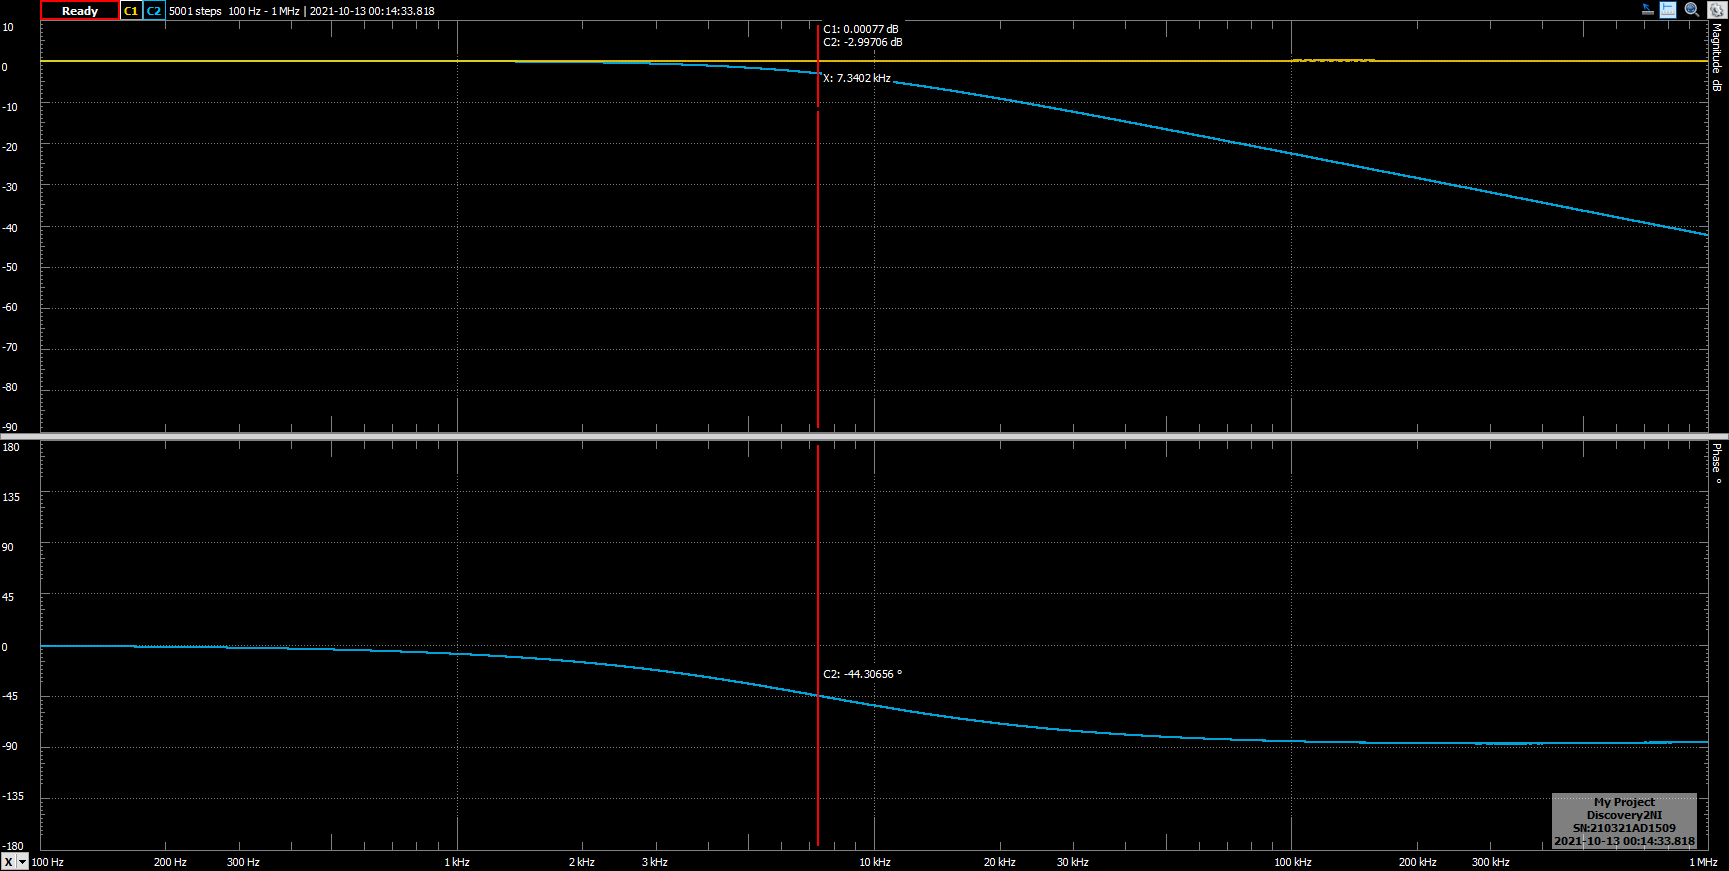
\includegraphics[scale=0.35]{rc2k10nF_new}
\caption{Plot di Bode per il filtro passa-basso.}
\end{figure}

\subsection*{5.a Stima della frequenza di taglio (metodo a)}
La nostra stima della frequenza per cui $A_v$(dB) = -3 dB \`e
\[
f_{1A} = 7336 \pm 6 \; \si{\Hz}
\]

\subsection*{5.b Misura della frequenza di taglio (metodo b)}
Dal fit a bassa frequenza ($f\ll f_1$) otteniamo
\[
A_1(\mathrm{dB}) = \left(-17.91 \pm 0.18\right)\times 10^{-3} \;\;\;
\chi^2 = 243 \;\;\; d.o.f. = 873
\]

Ad alta frequenza ($f \gg f_1$) la retta di best-fit al plot di Bode in 
ampiezza ha i seguenti parametri:
\[
\mathrm{intercetta} = 75.928 \pm 0.008 \;\;\;\mathrm{pendenza} = -19.6747 \pm 
0.0016 \;\;\;\mathrm{correlazione} 
= -0.997 \;\;\; \chi^2 = 1647 \;\;\; d.o.f. = 1746
\]
Dall'intersezione delle due rette stimiamo per la frequenza di taglio il valore
\[
f_{1B} = 7246 \pm 8 \; \si{Hz}
\]

\begin{figure}[htbp]
\centering
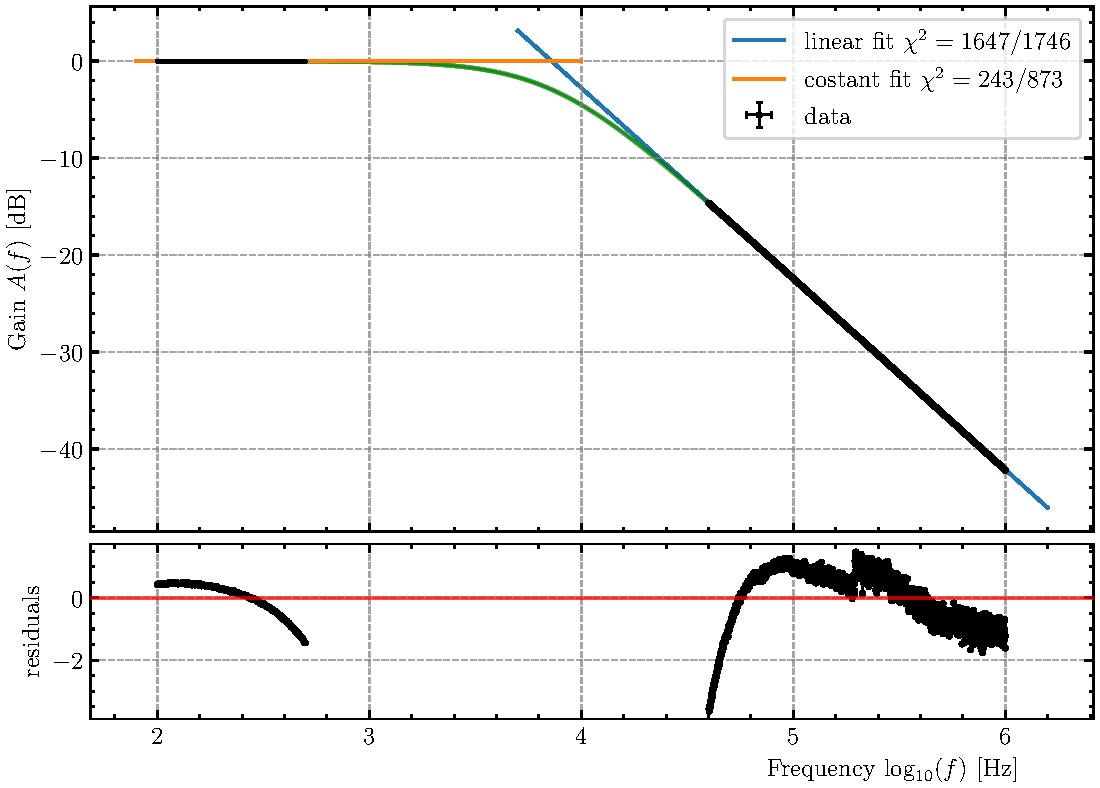
\includegraphics[scale=0.7]{corner}
\caption{Fit al plot di bode per trovare la frequenza di corner. In verde i
punti non utilizzati nel fit. \label{fig: corner}}
\end{figure}

\subsection*{5.c Misura della frequenza di taglio (metodo c)}
Dal fit complessivo del modulo della funzione di trasferimento
\begin{equation}\label{eq: lpfgain}
\abs{T(f)} = A(f) = \frac{1}{\sqrt{1 + \left(\frac{f}{f_1}\right)^2}}
\end{equation}
otteniamo per l'~amplificazione di centro-banda e per la frequenza di taglio i 
seguenti valori:
\[
A_1 (\mathrm{dB}) = \left(-19.1 \pm 0.3\right)\times 10^{-3} \;\;\;
f_{1C} = 7428.8 \pm 0.9 \si{\Hz} \;\;\;\ \chi^2 = 1614 \;\;\; d.o.f.= 4997
\]

\begin{figure}[htb]
\centering
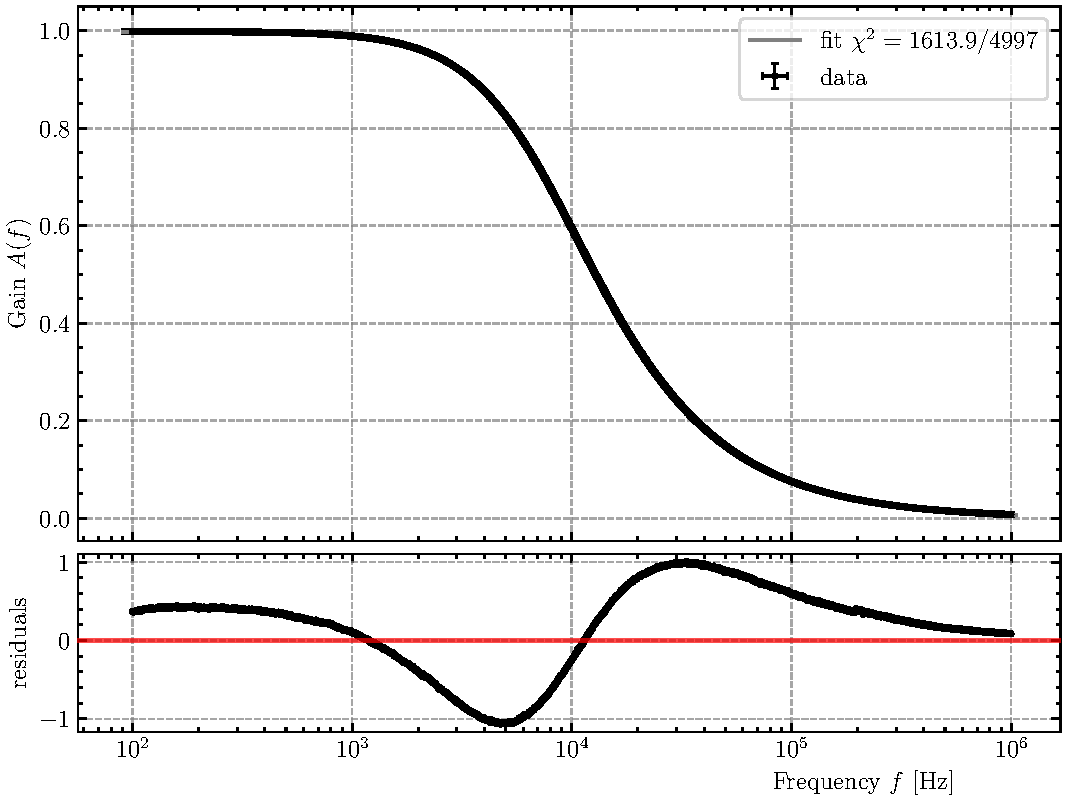
\includegraphics[scale=0.7]{lpfbodefit}
\caption{Fit complessivo al plot di bode con l'espressione per l'attenuazione
\eqref{eq: lpfgain}.\label{fig: lpfbodefit}}
\end{figure}


\subsection*{5.d Confronto misure-predizione}
Le misure delle frequenze di taglio trovate con i 3 diversi metodi sono tutte
compatibili con il valore atteso dalle misure di $R_1$ e $C_1$ visto in 1.f;
ma non compatibili entro le relative incertezze tra loro.
In particolare la misura più precisa è quella ottenuta tramite fit complessivo
(metodo c) mentre quella più vicina al valore atteso è quella ottenuta
direttamente dal plot di Bode generato dall'AD2 (metodo a).

\subsection*{6 Risposta del filtro ad un gradino}
Il fronte del segnale di uscita ha un tempo di salita, misurato con i cursori, 
di 
\[
t_r = 47 \pm 2 \; \si{\micro\second}
\]
da cui 
\[
f_1 = \ln(9) R_1 C_1 \approx \frac{2.2}{2\pi t_r} = 7.4 \pm 0.3 \; \si{k\Hz}
\]
\begin{figure}[htb]
\centering
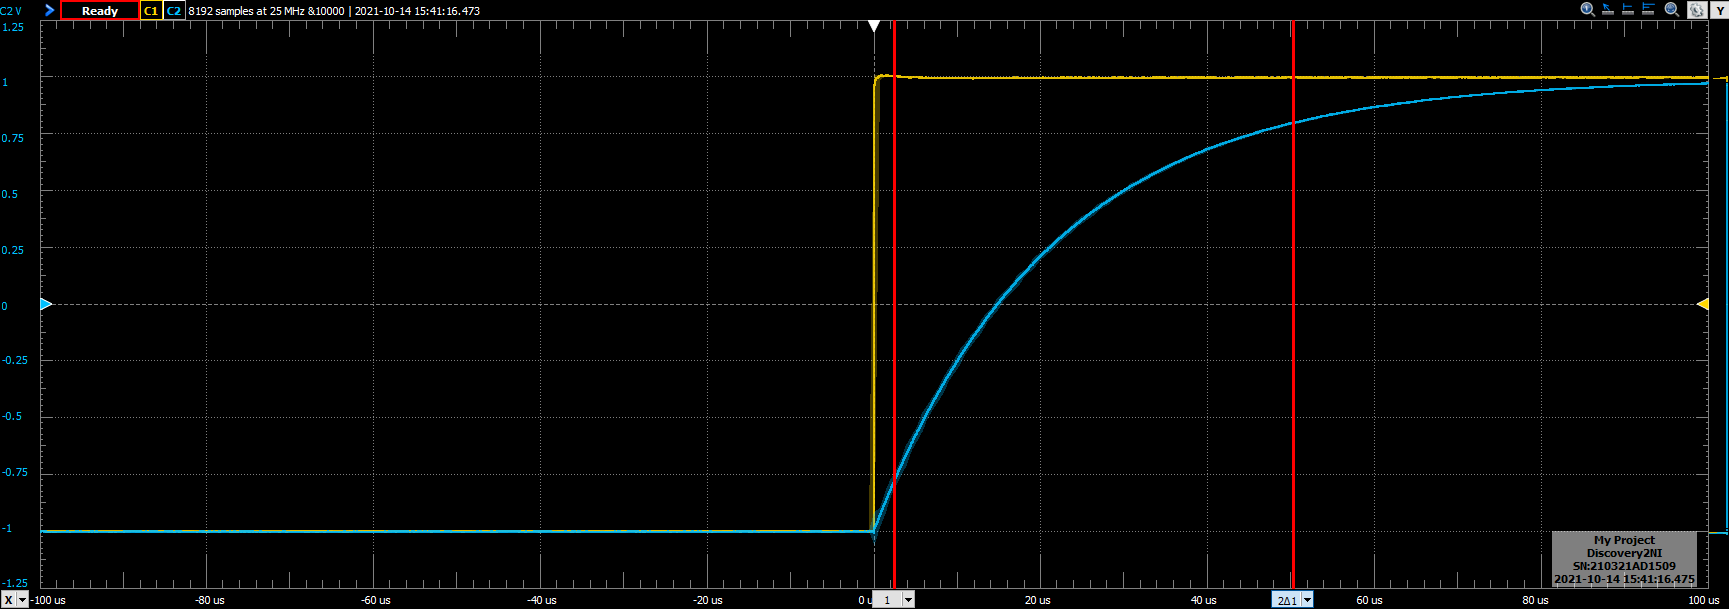
\includegraphics[scale=0.35]{rc2k10nF_rise}
\caption{(6) Risposta del filtro passa-basso ad un gradino di tensione.}
\end{figure}

\subsection*{7.a Impedenze di ingresso/uscita}
L'impedenza in ingresso al circuito in \ref{fig: lpfcirc} è data da:
\[
Z\ped{in}(\omega) = R_1 + \frac{1}{j \omega C_1} =
R_1 \left( 1 - j \frac{1}{\omega R_1 C_1} \right) =
R_1 \left( 1 - j \frac{\omega_1}{\omega} \right)
\]

A bassa frequenza ($f \ll f_1$) il termine costante è trascurabile, per cui
\[
Z\ped{in}(f) \approx -jR_1 \frac{f_1}{f}
\]
Poiché l'impedenza del condensatore $Z_{C_1} \to \infty$ per $f \to 0$
il filtro si comporta come un circuito aperto.

Ad alta frequenza ($f \gg f_1$) è il termine costante a dominare, quindi
\[
Z\ped{in} \approx R
\]
cioè, nel limite opposto ($Z_{C_1} \to 0$ per $f \to \infty$) il
condensatore si comporta come un corto-circuito, quindi il filtro ha
impedenza puramente reale.

Alla frequenza di taglio vale
\[
Z\ped{in} = R_1 (1 - j)
.\]

Mentre come impedenza in uscita abbiamo:
\[
Z\ped{out}(\omega) = \left(\frac{1}{R_1} + j\omega C_1\right)^{-1}
.\]

\subsection*{7.b Effetti dovuti all'~accoppiamento con un carico}
L'~amplificazione di centro-banda e la frequenza di taglio nel 
caso in cui il carico sia rispettivamente 100 e 10 k$\Omega$:
\[
\begin{array}{rl}
R_L=100 \,k\Omega & \implies A_1 = 0.98 \;\;\; f_1 = 7450 \; \si{\Hz} \\
R_L=10 \,k\Omega & \implies A_1 = 0.83\;\;\; f_1 = 8761 \; \si{\Hz} \\
\end{array}
\]

Si vede dal circuito equivalente di Thèvenin che la tensione ai capi del
condensatore è quella in uscita dal partitore di tensione
$V_{C_1} = R_L/(R_1 + R_L) V\ped{in} \implies A_1 = R_L/(R_1 + R_L)$ e che
la resistenza a cui si trova in serie $C_1$ è il parallelo $R_1 || R_2 =
(\frac{1}{R_1} + \frac{1}{R_2})^{-1} = \frac{R_1 R_2}{R_2 + R_1}$ che alza
la frequenza di taglio rispetto al valore atteso senza carico
$f_{1L} = \frac{1}{2\pi (R1 || R_2) C_1} \geq \frac{1}{2\pi R_1 C_1} = f_1$.

%=======================
\section*{Filtro passa-banda}

\subsection*{8.a Misura dei componenti}
\begin{align*}
R_1 = 1.98 \pm 0.02 \; \si{k\ohm} \quad C_1 = 10.8 \pm 0.4 \; \si{n\F} \quad
f_1 = 7442 \pm 351 \; \si{\Hz}
\end{align*}

\subsection*{8.b Filtro passa-basso, stima della frequenza di taglio}
Dalla fit con la funzione di trasferimento del passa basso risulta:
\begin{figure}[htb]
\centering
\includegraphics[scale=0.35]{passa_basso}
\caption{Fit con il modello della funzione di trasferimento per il filtro passa basso}
\end{figure}
Il valore della frequenza di taglio vale invece:
\begin{align*}
f_1 = 7.76 \pm 0.01 \; \si{k\Hz}\\
\end{align*}
che è compatibile con i valori attesi.

Il guadagno a centro banda vale:
\begin{align*}
A_1 = (-61 \pm 5) \times 10^{-3} \; \si{dB}
\end{align*}

\subsection*{9.a Misura dei componenti}
\begin{align*}
R_2 = 1.98 \pm 0.02 \; \si{k\ohm} \quad C_1 = 97.6 \pm 3.9 \; \si{n\F} \quad
f_1 = 821 \pm 41 \; \si{\Hz}
\end{align*}

\subsection*{9.b Filtro passa-alto, stima della frequenza di taglio}
Dal fit con modello la funzione di trasferimento di un filtro passa alto risulta:
\begin{figure}[htb]
\centering
\includegraphics[scale=0.35]{passa_alto}
\caption{Fit con il modello della funzione di trasferimento per il filtro passa alto}
\end{figure}
Il valore della frequenza di taglio ricavata dal fit vale:
\begin{align*}
f_2 = 821.3 \pm 0.2 \; \si{Hz}
\end{align*}
Il guadagno a centro banda vale:
\begin{align*}
A_2 = (-25.1 \pm 0.2) \times 10^{-3} \; \si{dB}
\end{align*}
\subsection*{10.a Filtro passa-banda, risposta in frequenza}
\begin{figure}[htb]
\centering
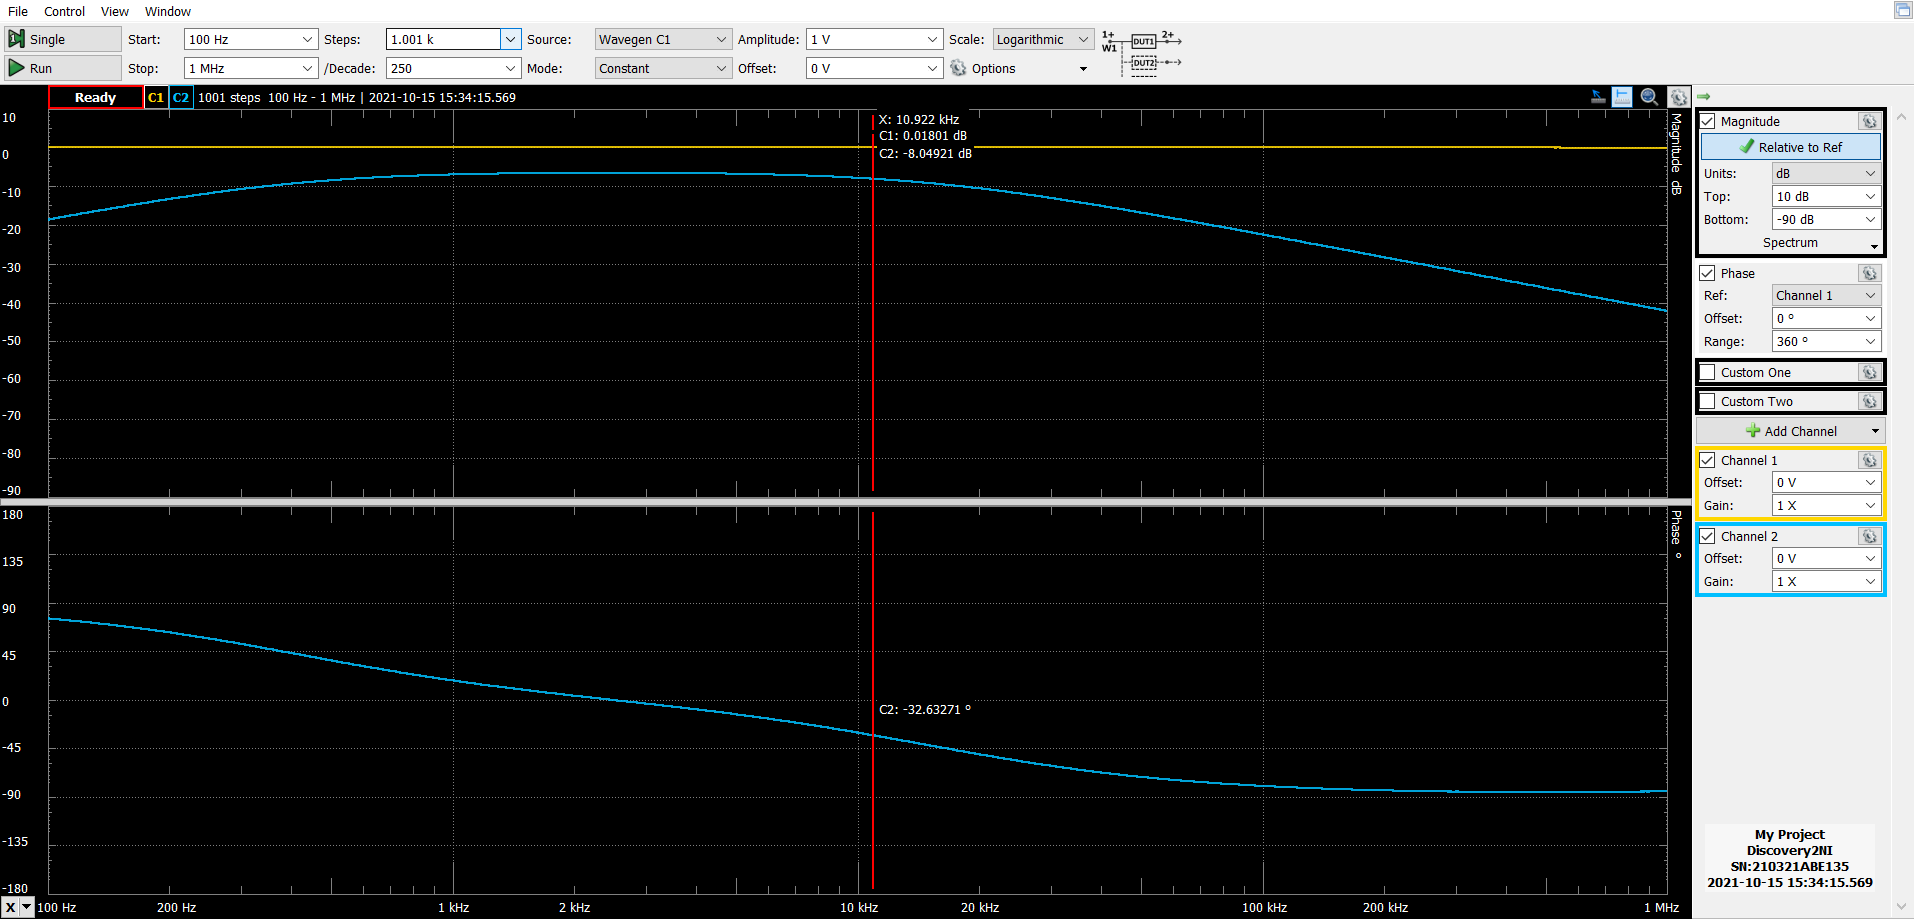
\includegraphics[scale=0.35]{passabanda}
\caption{(4) Immagine del network analyzer per il filtro passa-banda.}
\end{figure}
La nostra stima dell'amplificazione di centro-banda e delle frequenze di 
taglio (per cui il guadagno si riduce di 3 dB rispetto a centro-banda) \`e
\[
A(\mathrm{dB}) = -6.505 \pm 0.006 \;\;\; f_{L} = 380 \pm 4 \si{\Hz} \;\;\;
f_{H} = 16.29 \pm 0.16 \si{k\Hz}
\]

\subsection*{10.b Fit della funzione di trasferimento}
Utilizzando come modello il modulo della funzione di trasferimento per il passa banda $\frac{1}{\sqrt{(c + \frac{fa}{fb} + 1)^2 + (x/fb - fa/x)^2}}$ con $c=\frac{R1}{R2}$ si ottiene

\begin{figure}[htb]
\centering
\includegraphics[scale=0.35]{passa_banda}
\caption{Fit con il modello della funzione di trasferimento per il filtro
passa banda}
\end{figure}

\iffalse
Dal fit del plot di Bode in ampiezza si ha
\[
A(\mathrm{dB}) = \ldots \pm \ldots \;\;\;f_{L} = \ldots\pm \ldots\;\;\;f_{H} = 
\ldots\pm 
\ldots\;\;\;\chi^2 = \ldots\;\;\; d.o.f.= \ldots
\]
\fi
\subsection*{10.c Differenze}
A differenza dei circuiti RC studiati prima, non possiamo considerare
indipendenti i sotto-circuiti che compongono il passa-banda; infatti il
comportamento reale del circuito è sensibilmente diverso da quanto previsto in 
approssimazione di stadi indipendenti.

In particolare a centro banda (i.e. nell'intervallo di frequenza
$f_2 \leq f \leq f_1$) l'attenuazione non è più in ottima approssimazione
unitaria, ma è minore di $A\ped{max}(f) \approx \SI{-6}{\dB/dec}$.

Le frequenze di taglio misurate $f_L$ e $f_H$ non sono compatibili con quelle
ottenute separatamente nell'analisi dei singoli circuiti. Più precisamente
la frequenza più bassa (del passa alto) è pressoché dimezzata
$f_L > f_2$, mentre la frequenza più alta (del passa basso) è più che
raddoppiata $f_H > f_1$.

D'altra parte, una ragionevole richiesta per assicurare l'indipendenza dei due
circuiti collegati in serie è che si abbia
$\abs{Z\ped{out, 1}} \ll \abs{Z\ped{in,2}}$ ad ogni frequenza (e 
indipendentemente da questa). Riportiamo le impedenze in questione:
\[
\abs{Z\ped{out, 1}} = \abs{\frac{R_1}{1 + j \omega R_1 C_1}}^2 = 
\frac{R_1^2}{1 + \omega^2 R_1^2 C_1^2}
\qquad
\abs{Z\ped{in, 2}}^2 = \abs{\frac{1 + j \omega R_2 C_2}{j\omega 
C_2}}^2 = \frac{1 + \omega^2 R_2^2 C_2^2}{\omega^2 C_2^2}
\]
Ora $\abs{Z\ped{out, 1}} \leq 1/(\omega C_1)$ con $\abs{Z\ped{out, 
1}} \sim 1/(\omega C_1)$ per $f \gg f_1 $ e $\abs{Z\ped{in, 2}} 
\geq 1/(\omega C_2)$ con $\abs{Z\ped{out, 1}} \sim 1/(\omega C_2) 
$ per $ f \ll f_2 $. Quindi per poter considerare indipendenti i due circuiti
è sicuramente una buona idea imporre la condizione
\[
\abs{Z\ped{out, 1}} \leq \frac{1}{\omega C_1} \ll \frac{1}{\omega C_2} \leq 
\abs{Z\ped{in, 2}} \implies C_2 \ll C_1.
\]
Mentre per i valori di capacità scelti vale la condizione opposta
$C_2 \approx 10 \cdot C_1$.

\subsection*{10.d Dipendenza dai valori delle resistenze}
Se indichiamo con $A_1(f)$ e $A_2(f)$ le attenuazioni del passa-basso e del
passa-alto, l'attenuazione attesa in uscita dai due circuiti collegati in
cascata è
\begin{equation}\label{eq: bpfgain}
A = \left(\frac{R_1}{R_2} + \frac{1}{A_1 A_2}\right)^{-1} = 
\frac{A_1 A_2}{A_1 A_2 \frac{R_1}{R_2} + 1} 
\end{equation}
Nel nostro caso vale $R_1 = R_2$ (entro l'incertezza) per cui come
attenuazione di centro banda, dove avevamo $A_1 \approx A_2 \approx 1$, ci
aspettiamo di avere $A\ped{cb} = \frac{1}{2}$.
Questo è compatibile con il valore che abbiamo misurato (prima in dB)
$A\ped{cb} = 0.4702 \pm 0.0004 \approx \frac{1}{2}$

Per avere una risposta in frequenza del circuito complessivo il più possibile
uguale al prodotto delle funzioni di trasferimento dei due sotto-circuiti
avremmo dovuto scegliere $R_1 \ll R_2$ ($Z\ped{out, 1} \ll Z\ped{in, 2}$.
Infatti l'attenuazione attesa a centro banda vista in \eqref{eq: bpfgain}
sotto queste ipotesi diventa $A\ped{cb} \approx A_1 A_2 \approx 1$.
\subsection*{10.e Andamento della fase}
Idealmente, se la funzione di trasferimento complessiva $T(\omega)$ per il
passa banda è il prodotto delle funzioni di trasferimento dei due circuiti in
cascata:
\begin{align*}
T_1(\omega) = -\frac{1}{1 + j \omega/\omega_1} \qquad
T_2(\omega) = \frac{1}{1 - j \omega_2/\omega}
\end{align*}
ci aspettiamo (per le regole di moltiplicazione sui complessi) che lo
sfasamento totale in uscita sia pari alla somma degli sfasamenti prodotti dai
singoli sotto-circuiti:
\[
T(\omega) = T_1(\omega) T_2(\omega) =
\abs{T_1} e^{i (\omega t + \phi_1)} \abs{T_2} e^{i (\omega t + \phi_2)} =
\abs{T_1} \abs{T_2} e^{i (\omega t + \phi_1 + \phi_2)} =
\abs{T_1} \abs{T_2} e^{i (\omega t + \phi)}
\]
per cui $\phi = \phi_1 + \phi_2 =
\tan^{-1} \left( \dfrac{\Im{\{T_1(\omega)\}}}{\Re{\{T_1(\omega)\}}} \right) +
\tan^{-1} \left( \dfrac{\Im{\{T_2(\omega)\}}}{\Re{\{T_2(\omega)\}}} \right)$
che corrispondono rispettivamente a
\begin{align*}
\phi_1(\omega) = \arctan - \frac{\omega}{\omega_1} \qquad
\phi_2(\omega) = \arctan \frac{\omega_2}{\omega}
\end{align*}

Effettivamente le misure di sfasamento in uscita dal passa-banda risultano
in accordo con l'andamento atteso
\begin{equation}
\phi_2 + \phi_1 = \phi(f) = \arctan{\frac{f_2}{f}} - \arctan{\frac{f}{f_1}}
\end{equation}
\begin{figure}[htb]
\centering
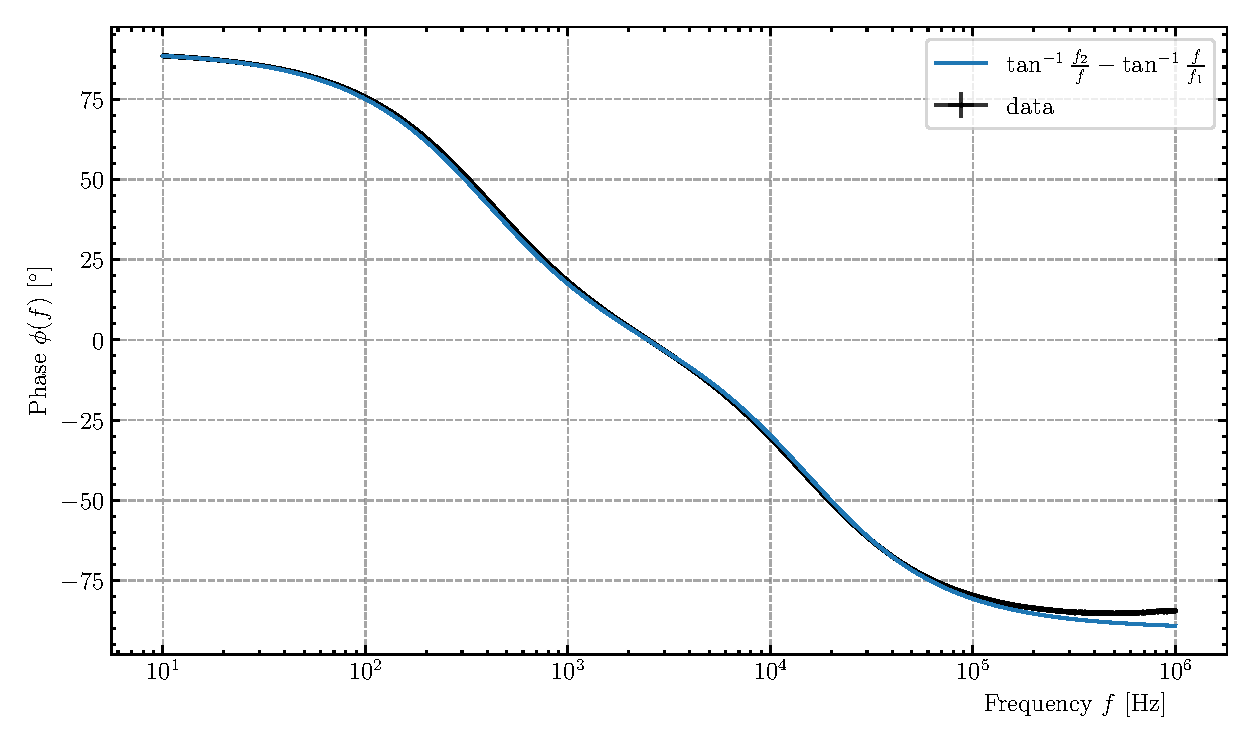
\includegraphics[scale=0.7]{bpfphase}
\caption{Grafico dello sfasamento misurato per il filtro passa-banda al
variare della frequenza in scala semilogaritmica.}
\end{figure}
almeno fino a frequenze dell'ordine di $10^5 \; \si{\Hz}$ dove i punti
iniziano a deviare dal modello man mano che ci si avvicina alla banda
passante dell'AD2 $(\sim 9 \; \si{M\Hz})$. Questo può essere dovuto alle
capacità parassite tra i fili, i componenti e la basetta che ad alta
frequenza non sono trascurabili, a differenza di quanto presuppone il nostro
modello.

\section*{Conclusioni e commenti finali}
Si è riusciti a realizzare dei filtri RC passivi del primo ordine
(o ``a un polo'') e ad apprezzarne il differente comportamento in vari
regimi, quando usati separatamente, collegati in cascata e connessi a
carichi resistivi di diverso valore.
\iffalse
\begin{figure}[htb]
\centering
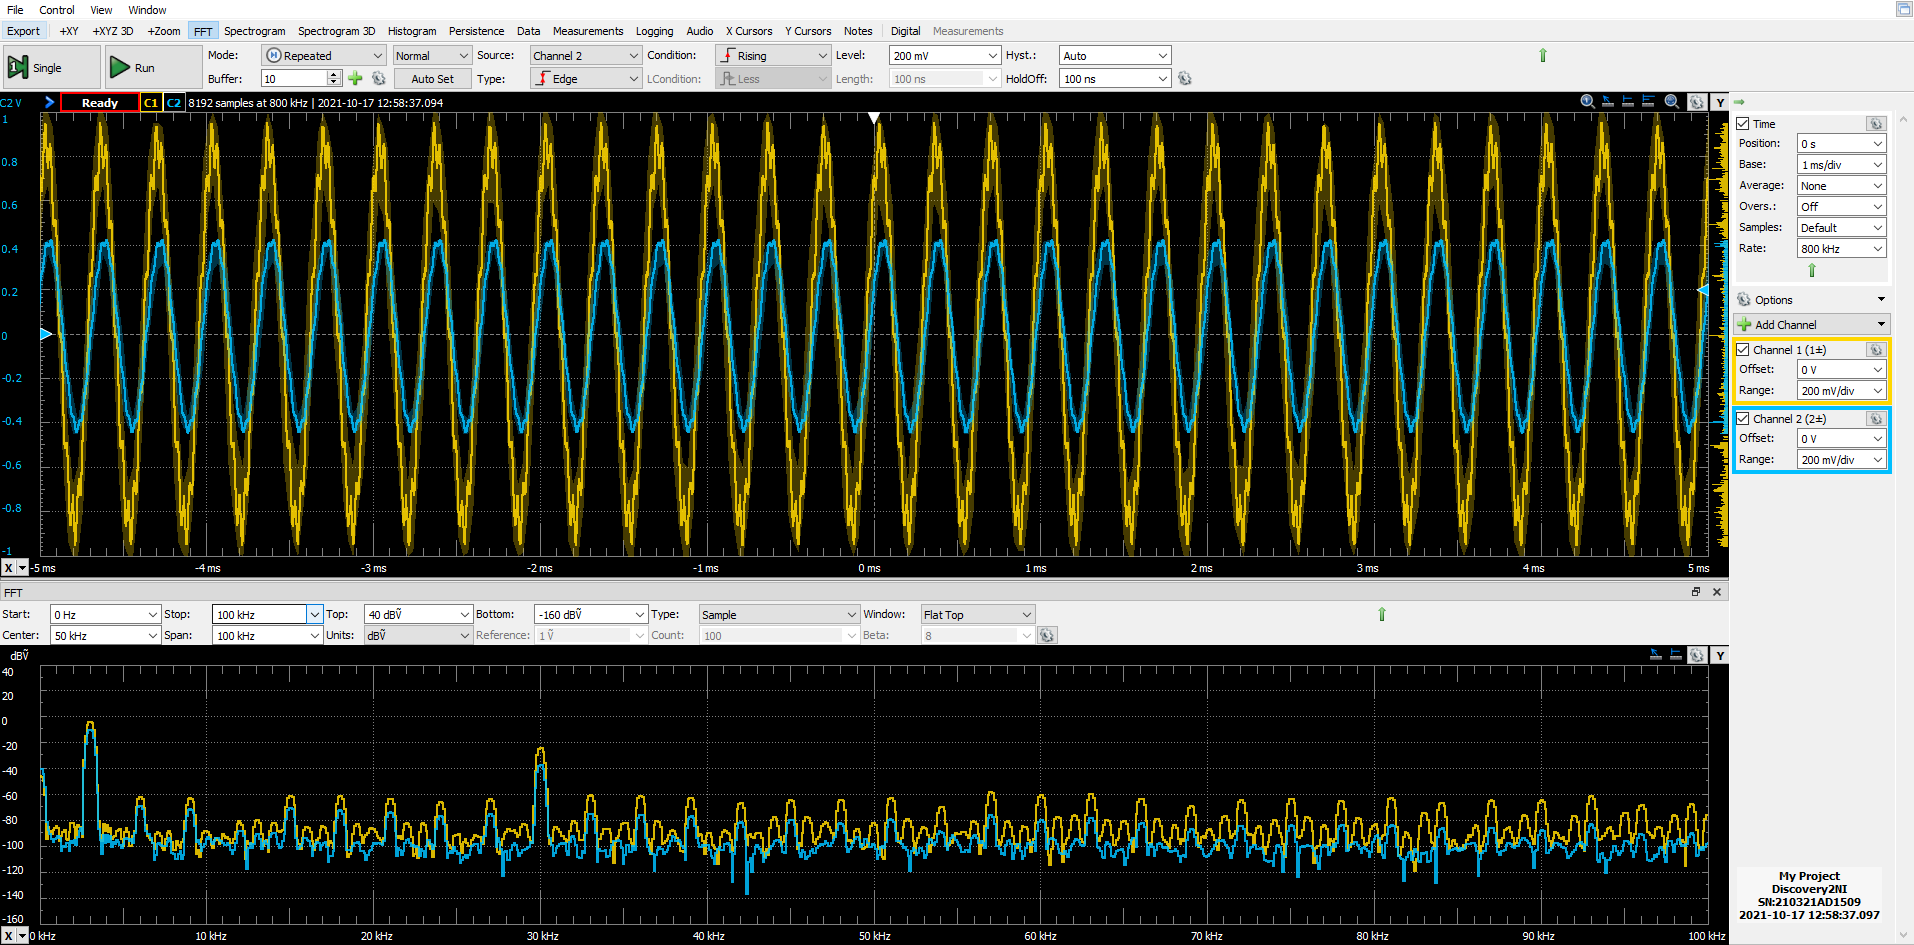
\includegraphics[scale=0.33]{noisine}
\caption{Sia nel dominio del tempo che delle frequenze si vede come il filtro
passa-basso progettato riesca ad attenuare sensibilmente il rumore a
$\SI{30}{k\Hz}$ sovrapposto al segnale portante di frequenza $\SI{3}{k\Hz}$.}
\end{figure}
\fi

\section*{Dichiarazione}
I firmatari di questa relazione dichiarano che il contenuto della relazione \`e 
originale, con misure effettuate dai membri del gruppo, e che tutti i firmatari 
hanno contribuito alla elaborazione della relazione stessa.

\end{document}
